\section{Paper A: AES for Heston-Type Models}

\begin{frame}{Paper A: AES for Heston-Type Models}
  \keymessage{Paper A extends the Almost-Exact Simulation scheme to Bermudan and American put options under Heston and double Heston models.}

  \vspace{0.5em}
  \begin{columns}[T,onlytextwidth]
    \begin{column}{0.47\textwidth}
      \begin{block}{The idea}
        \begin{itemize}
          \item Sample each CIR variance factor from its noncentral chi-square distribution.
          \item Use the sampled variance values in the log-price update.
          \item Avoid the negative variance values that may appear in standard Euler discretization.
        \end{itemize}
      \end{block}
    \end{column}
    \begin{column}{0.47\textwidth}
      \begin{block}{Terminology}
        AES is not fully exact. It is almost exact because remaining stochastic integrals in the log-price update are still approximated.
      \end{block}
      \begin{block}{Role in early-exercise pricing}
        Paper A reports higher accuracy and computational efficiency when the number of simulation steps matches the exercise dates for Bermudan options.
      \end{block}
    \end{column}
  \end{columns}
\end{frame}

\begin{frame}{Paper A Derivation: Double Heston AES One-Step Update}
  \vspace{-0.2em}
  \begin{columns}[T,onlytextwidth]
    \begin{column}{0.49\textwidth}
      \begin{block}{1. Double Heston log-price form}
        {\fontsize{4.0}{4.45}\selectfont
        \setlength{\abovedisplayskip}{1pt}
        \setlength{\belowdisplayskip}{1pt}
        Applying It\^{o}'s lemma to \(X_t:=\ln S_t\) and a Cholesky
        decomposition gives
        \[
        \resizebox{0.74\linewidth}{!}{$
        \begin{aligned}
        \dd X_t&=\left(r-\frac12(\nu_t^1+\nu_t^2)\right)\dd t
        +\sqrt{\nu_t^1}\left(\rho_{1,3}\dd\widetilde W_t^3
        +\sqrt{1-\rho_{1,3}^2}\dd\widetilde W_t^1\right)\\
        &\quad+\sqrt{\nu_t^2}\left(\rho_{2,4}\dd\widetilde W_t^4
        +\sqrt{1-\rho_{2,4}^2}\dd\widetilde W_t^2\right),\\[-0.15em]
        \dd\nu_t^1&=\kappa_1(\bar\nu_1-\nu_t^1)\dd t+
        \gamma_{v_1}\sqrt{\nu_t^1}\dd\widetilde W_t^3,\\[-0.15em]
        \dd\nu_t^2&=\kappa_2(\bar\nu_2-\nu_t^2)\dd t+
        \gamma_{v_2}\sqrt{\nu_t^2}\dd\widetilde W_t^4 .
        \end{aligned}
        $}
        \]
        The four \(\widetilde W\)-increments are independent.}
      \end{block}
      \begin{block}{2. Sample the two variance factors}
        {\tiny
        \[
        \nu_{j+1}^{(i)}=\bar c^{(i)}\chi^2_{\delta^{(i)}}\!\left(\bar\kappa^{(i)}\right),\quad i=1,2,
        \]
        \[
        \bar c^{(i)}=\frac{\gamma_{\nu_i}^2}{4\kappa_i}(1-e^{-\kappa_i\Delta t}),\quad
        \bar\kappa^{(i)}=\frac{4\kappa_i\nu_j^{(i)}e^{-\kappa_i\Delta t}}{\gamma_{\nu_i}^2(1-e^{-\kappa_i\Delta t})},
        \]
        \[
        \delta^{(i)}=\frac{4\kappa_i\bar\nu_i}{\gamma_{\nu_i}^2}.
        \]}
      \end{block}
    \end{column}
    \begin{column}{0.49\textwidth}
      \begin{block}{3. Constants used in the log-price update}
        {\tiny
        \[
        \begin{aligned}
        c_0&=\left(r-\frac{\rho_{1,3}\kappa_1\bar\nu_1}{\gamma_{\nu_1}}-\frac{\rho_{2,4}\kappa_2\bar\nu_2}{\gamma_{\nu_2}}\right)\Delta t,\\
        c_1&=\left(\frac{\rho_{1,3}\kappa_1}{\gamma_{\nu_1}}-\frac12\right)\Delta t-\frac{\rho_{1,3}}{\gamma_{\nu_1}},\quad
        c_2=\left(\frac{\rho_{2,4}\kappa_2}{\gamma_{\nu_2}}-\frac12\right)\Delta t-\frac{\rho_{2,4}}{\gamma_{\nu_2}},\\
        c_3&=\frac{\rho_{1,3}}{\gamma_{\nu_1}},\quad
        c_4=\frac{\rho_{2,4}}{\gamma_{\nu_2}},\quad
        c_5=(1-\rho_{1,3}^2)\Delta t,\quad
        c_6=(1-\rho_{2,4}^2)\Delta t .
        \end{aligned}
        \]}
      \end{block}
      \begin{block}{4. Almost-exact asset update}
        {\tiny
        \[
        \begin{aligned}
        X_{j+1}&=X_j+c_0+c_1\nu_j^{(1)}+c_2\nu_j^{(2)}
        +c_3\nu_{j+1}^{(1)}+c_4\nu_{j+1}^{(2)}\\
        &\quad+\sqrt{c_5\nu_j^{(1)}}\,(W_{j+1}^{(1)}-W_j^{(1)})
        +\sqrt{c_6\nu_j^{(2)}}\,(W_{j+1}^{(2)}-W_j^{(2)}).
        \end{aligned}
        \]}
        {\scriptsize Finally set \(S_j=\exp(X_j)\).}
      \end{block}
    \end{column}
  \end{columns}
\end{frame}

\begin{frame}{Paper A: Bermudan Heston Numerical Results}
  \begin{columns}[T,onlytextwidth]
    \begin{column}{0.49\textwidth}
      \centering
      {\large\bfseries 40 exercise dates}\\[0.25em]
      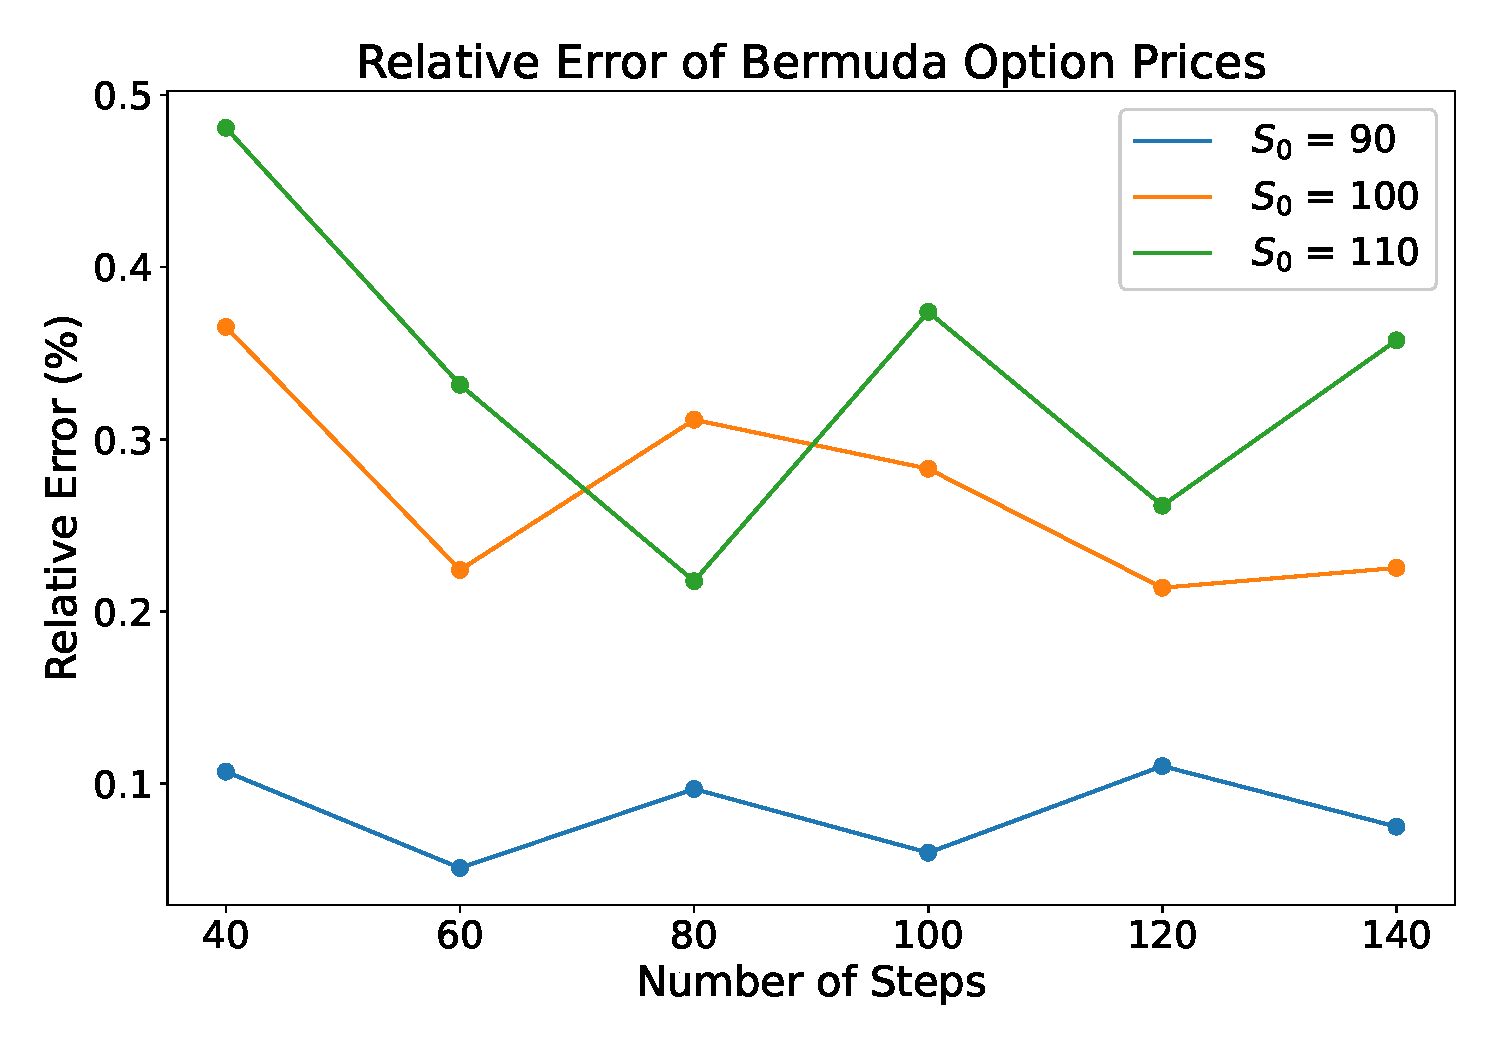
\includegraphics[width=\linewidth,height=0.56\textheight,keepaspectratio]{../Figures/PaperA/RelativeErrorsTable4_Bermudan_N=40_GlobalPolynomials2.pdf}
    \end{column}
    \begin{column}{0.49\textwidth}
      \centering
      {\large\bfseries 60 exercise dates}\\[0.25em]
      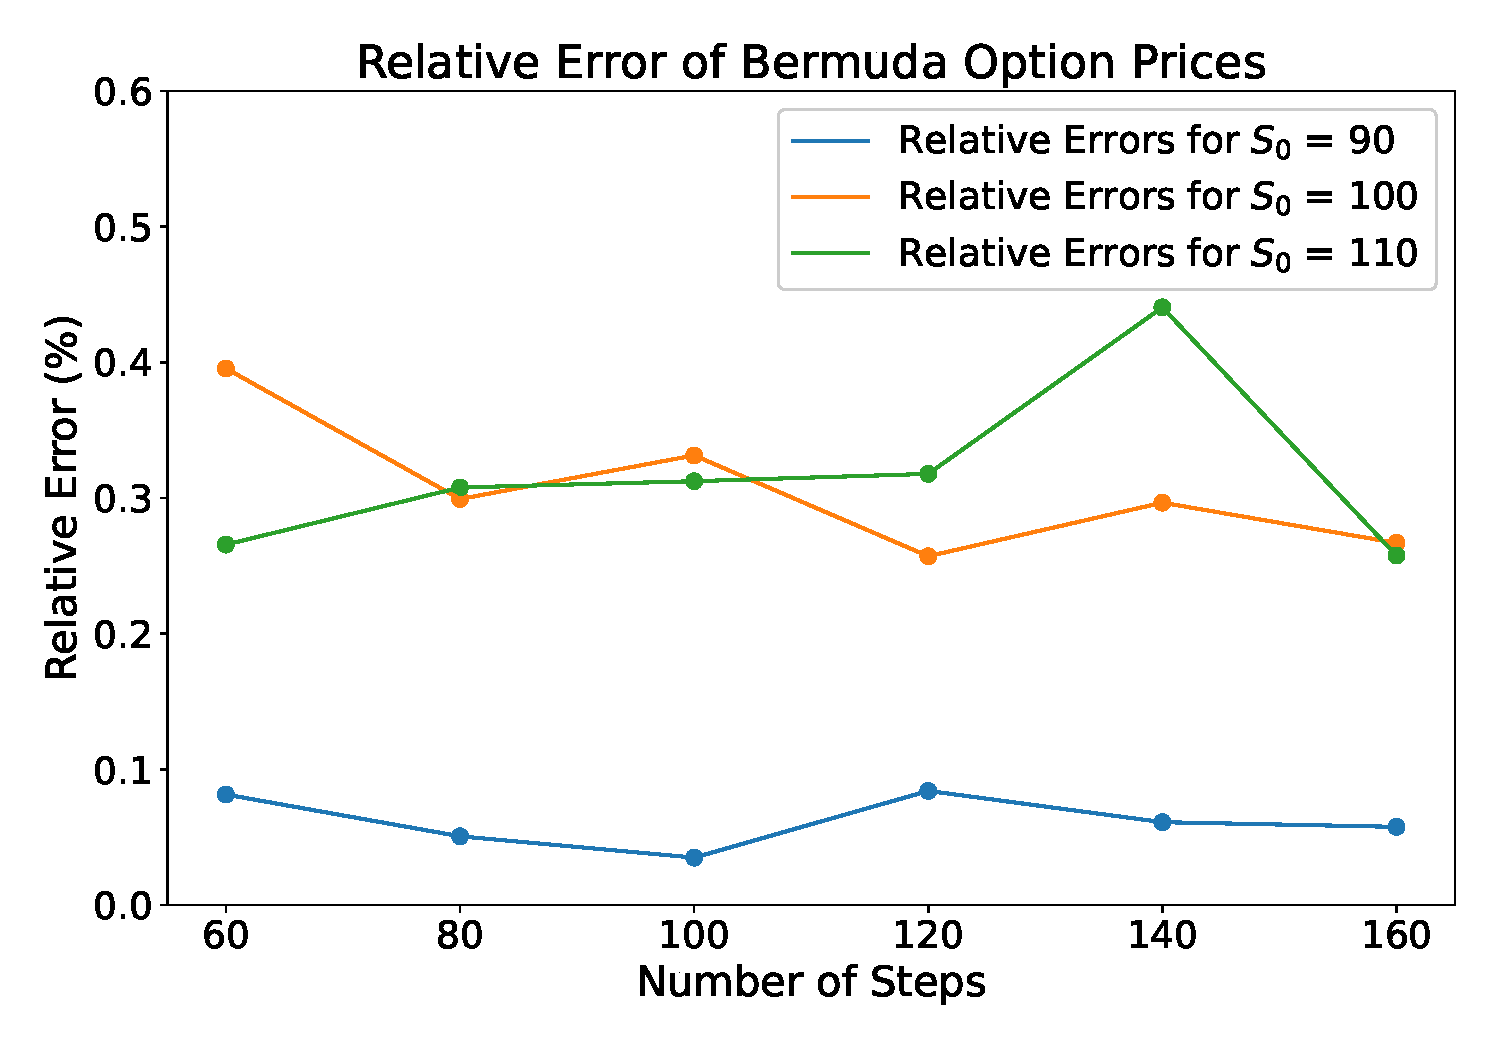
\includegraphics[width=\linewidth,height=0.56\textheight,keepaspectratio]{../Figures/PaperA/RelativeErrorsTable4_Bermudan_N=60_GlobalPolynomials2.pdf}
    \end{column}
  \end{columns}

  \vspace{0.25em}
  \keymessage{\footnotesize With simulation steps matched to exercise dates, AES yields low relative errors, especially for in-the-money and at-the-money puts.}
\end{frame}

\begin{frame}{Paper A: American Put Experiment}
  \begin{columns}[T,onlytextwidth]
    \begin{column}{0.46\textwidth}
      \begin{block}{Expertiment}
        \small        
        AES for Double Heston American put with \(M=12\) simulation steps and three test cases.
        The comparison is between AES and Euler with the same time-steps,
        and reference values.
      \end{block}
    \end{column}
    \begin{column}{0.50\textwidth}
      \centering
      \scriptsize
      \begin{tabular}{lccc}
        \toprule
        Method & Case 1 & Case 2 & Case 3\\
        \midrule
        AES, \(M=12\) & 6.992 & 9.635 & 12.676\\
        Euler, \(M=12\) & 5.116 & 7.611 & 10.608\\
        Reference & 6.887 & 9.504 & 12.520\\
        \bottomrule
      \end{tabular}
      \vspace{0.7em}
      \keymessage{\footnotesize At the same small number of simulation steps,
      AES is close to the reference values, while Euler is materially below the
      reference values in all three cases.}
    \end{column}
  \end{columns}
\end{frame}

\begin{frame}{Paper A: Efficiency Comparison}
  \begin{columns}[T,onlytextwidth]
    \begin{column}{0.33\textwidth}
      \centering
      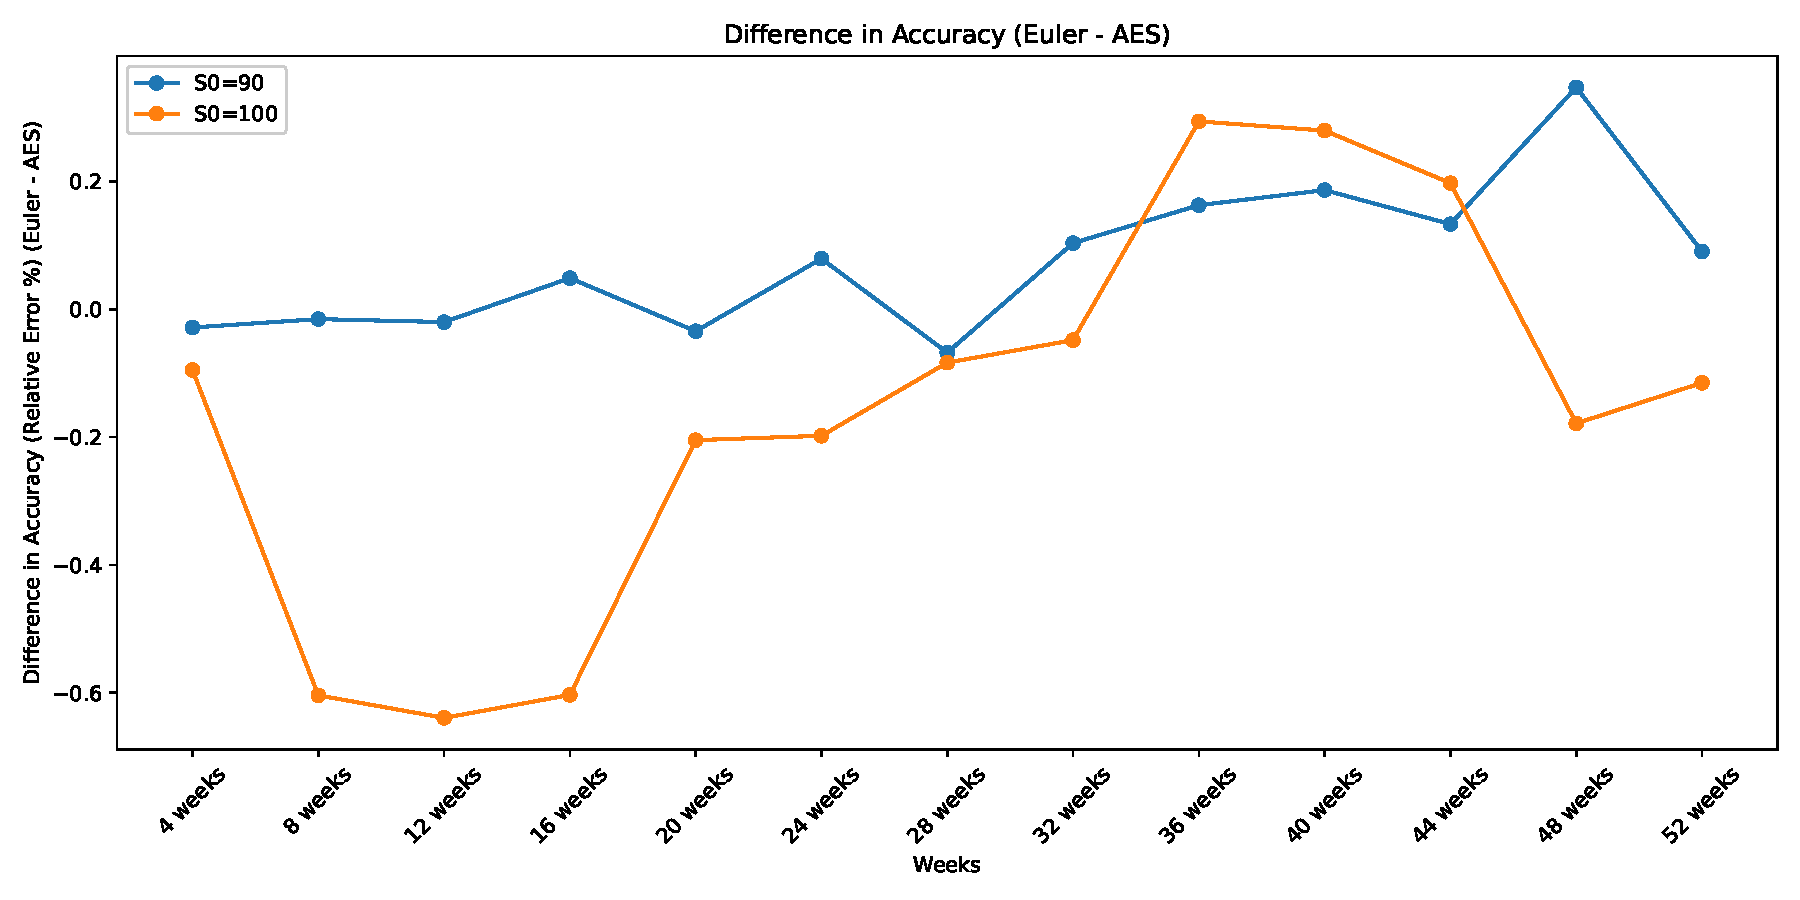
\includegraphics[width=\linewidth,height=0.58\textheight,keepaspectratio]{../Figures/PaperA/accuracy_difference2x.pdf}
      \tightcaption{Accuracy difference.}
    \end{column}
    \begin{column}{0.33\textwidth}
      \centering
      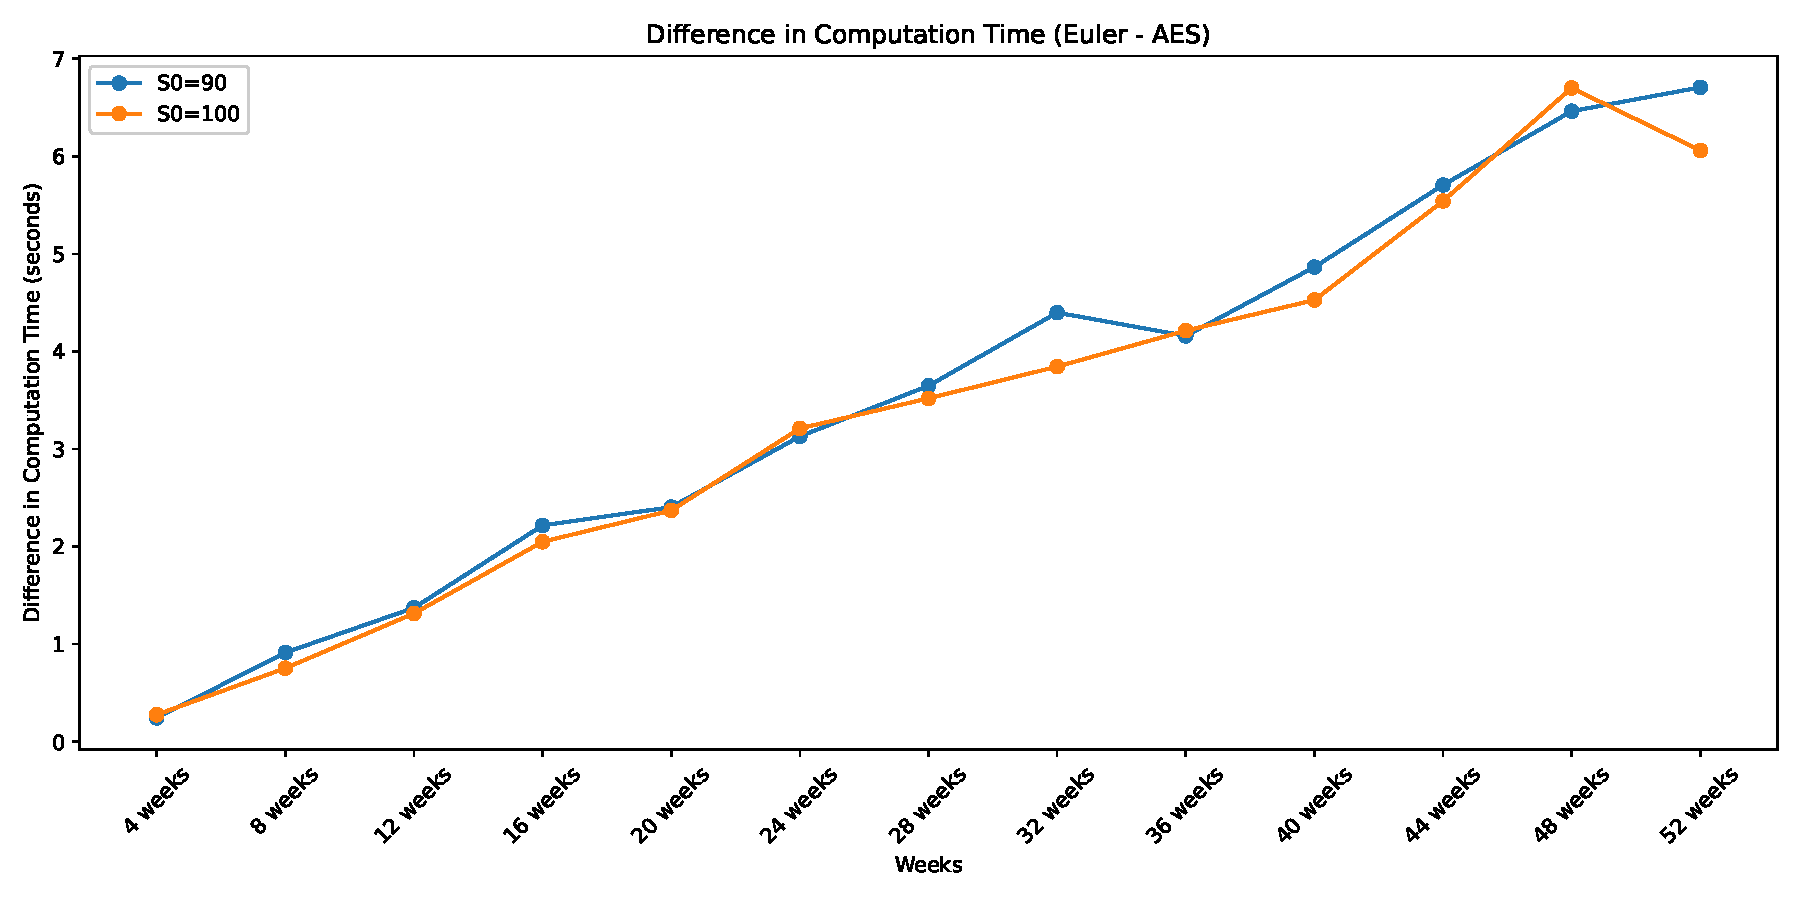
\includegraphics[width=\linewidth,height=0.58\textheight,keepaspectratio]{../Figures/PaperA/computation_time_difference2x.pdf}
      \tightcaption{Computation time.}
    \end{column}
    \begin{column}{0.33\textwidth}
      \centering
      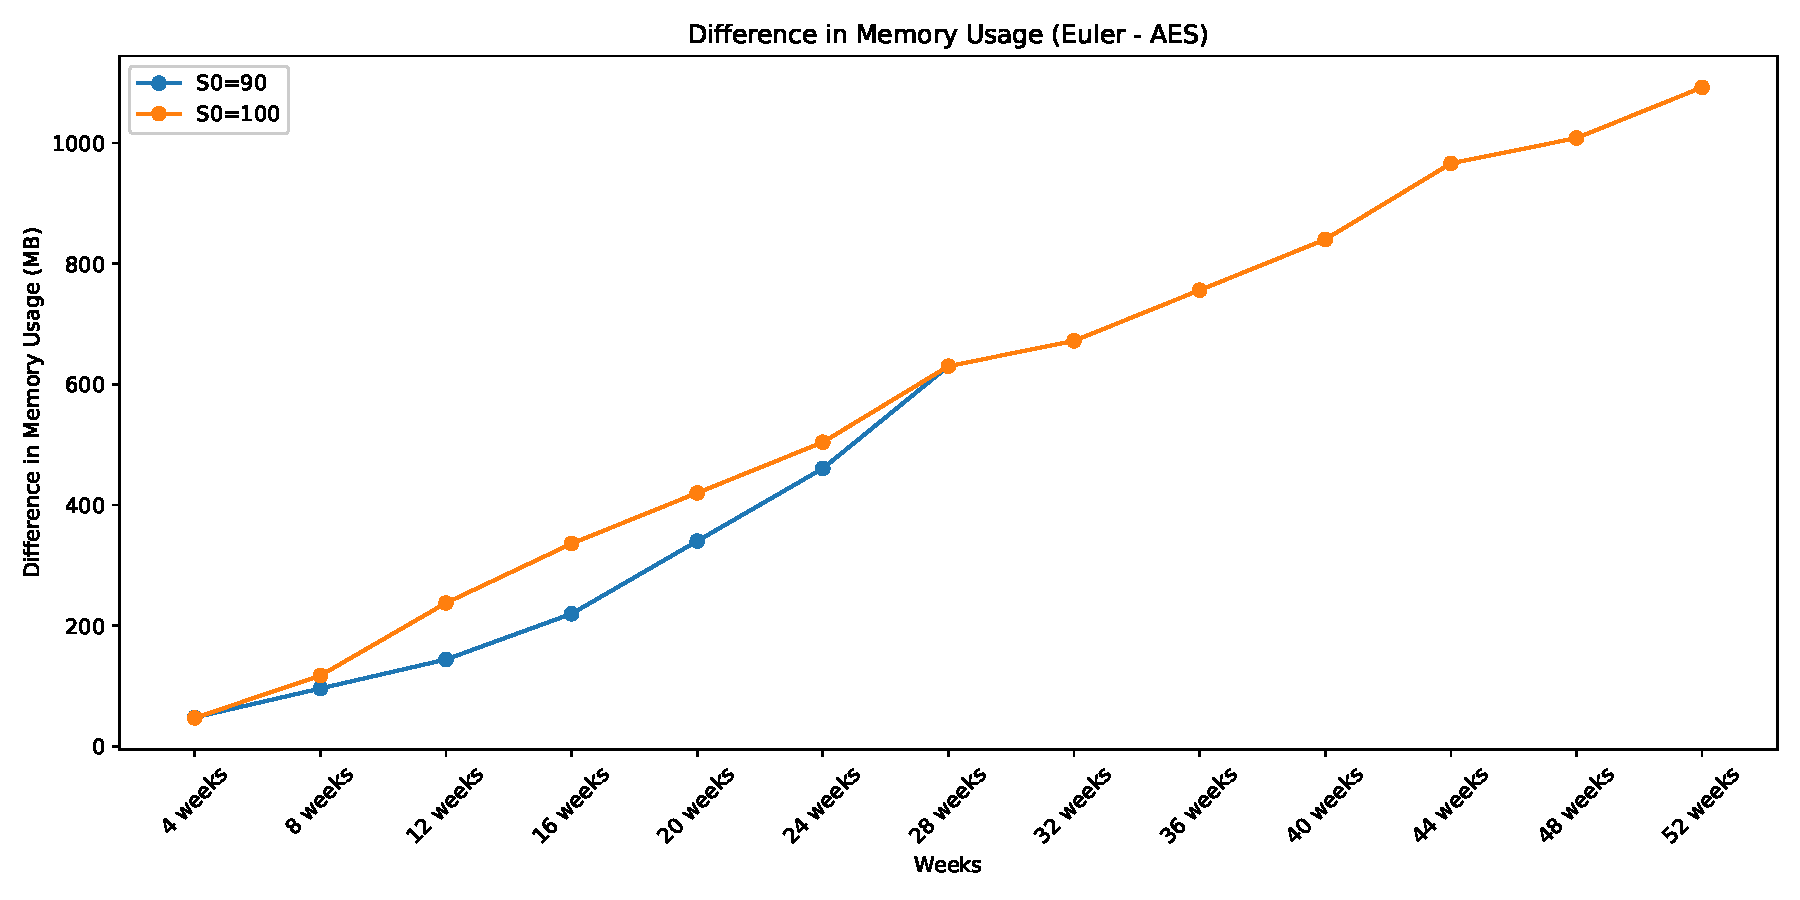
\includegraphics[width=\linewidth,height=0.58\textheight,keepaspectratio]{../Figures/PaperA/memory_usage_difference2x.pdf}
      \tightcaption{Memory usage.}
    \end{column}
  \end{columns}

  \vspace{0.3em}
  \keymessage{AES is useful when Euler requires additional time steps to reach comparable accuracy; in these cases AES can reduce computation time and memory use.}
\end{frame}

\begin{frame}{Paper A: Double Heston American Put Results}
  \centering
  \vspace{0.2em}
  {\small\bfseries Double Heston American put experiment with \(M=12\) simulation steps}\\[0.6em]
  \begin{tabular}{lccc}
    \toprule
    Method & Case 1 & Case 2 & Case 3 \\
    \midrule
    AES, \(M=12\) & 6.992 & 9.635 & 12.676 \\
    Euler, \(M=12\) & 5.116 & 7.611 & 10.608 \\
    Reference & 6.887 & 9.504 & 12.520 \\
    \bottomrule
  \end{tabular}

  \vspace{1.0em}
  \begin{beamercolorbox}[rounded=true,sep=0.9ex,wd=0.82\linewidth]{keybox}
    \small In all three cases, AES is close to the reference value, while Euler is visibly below the reference value at the same small number of time steps.
  \end{beamercolorbox}
\end{frame}

\begin{frame}{Paper A: Contribution and Limitations}
  \begin{columns}[T,onlytextwidth]
    \begin{column}{0.48\textwidth}
      \begin{block}{Strengths}
        \begin{itemize}
          \item The AES scheme is extended to Bermudan and American put options.
          \item The double Heston version is derived analytically.
          \item The strongest numerical evidence appears for in-the-money and at-the-money options.
        \end{itemize}
      \end{block}
    \end{column}
    \begin{column}{0.48\textwidth}
      \begin{block}{Limitations}
        \begin{itemize}
          \item Out-of-the-money cases with few exercise opportunities are less uniform.
          \item Heston and double Heston have CIR variance factors, which makes AES naturally applicable.
          \item Better path simulation does not remove the continuation-value approximation problem.
        \end{itemize}
      \end{block}
    \end{column}
  \end{columns}

  \vspace{0.45em}
  \begin{center}
    \small Paper B moves to Gatheral's double mean-reverting model, where the long-run variance level is itself stochastic.
  \end{center}
\end{frame}
